\chap{Modelo SIR}{SIR}
\graphicspath{{figs/cap2}}

\sect{Historia}{historia}

Desde tiempos remotos las epidemias y pandemias han sido origen de sufrimiento para la humanidad. Cada individuo, pueblo, ciudad o civilización amenazada por una epidemia ha tenido 
que enfrentarlas de una u otra manera. La historia de la humanidad está llena de acontecimientos epidemiológicos que han causado grandes pérdidas de vidas humanas y cambios en la 
forma de vida de las sociedades. La peste negra, la gripe española, la viruela, la tuberculosis, la malaria  y la fiebre amarilla,
entre otras, han sido algunas de las epidemias más devastadoras de la historia. 

\subsection*{Peste Negra}

En la Edad Media, la peste negra, que se extendió por Europa entre 1346 y 1353, causó la muerte de entre un tercio y la mitad de la población europea. La enfermedad 
se transmitía por medio de la picadura de pulgas infectadas que vivían en las ratas. De hecho, el mecanismo de transmisión de la enfermedad fue un misterio durante mucho tiempo.
En 1855, una epidemia de peste bubónica comenzó en el sur de China. Fue entonces cuando pudieron obtenerse resultados de laboratorio y recién en 1897, M. Ogata, y en 1898,
P. L. Simonds, de manera independiente llegaron a la hipótesis de que la enfermedad se transmitía por medio de la picadura de pulgas infectadas. Lo cual fue confirmado unos 
años más tarde. 


\begin{figure}[h]
    \centering
    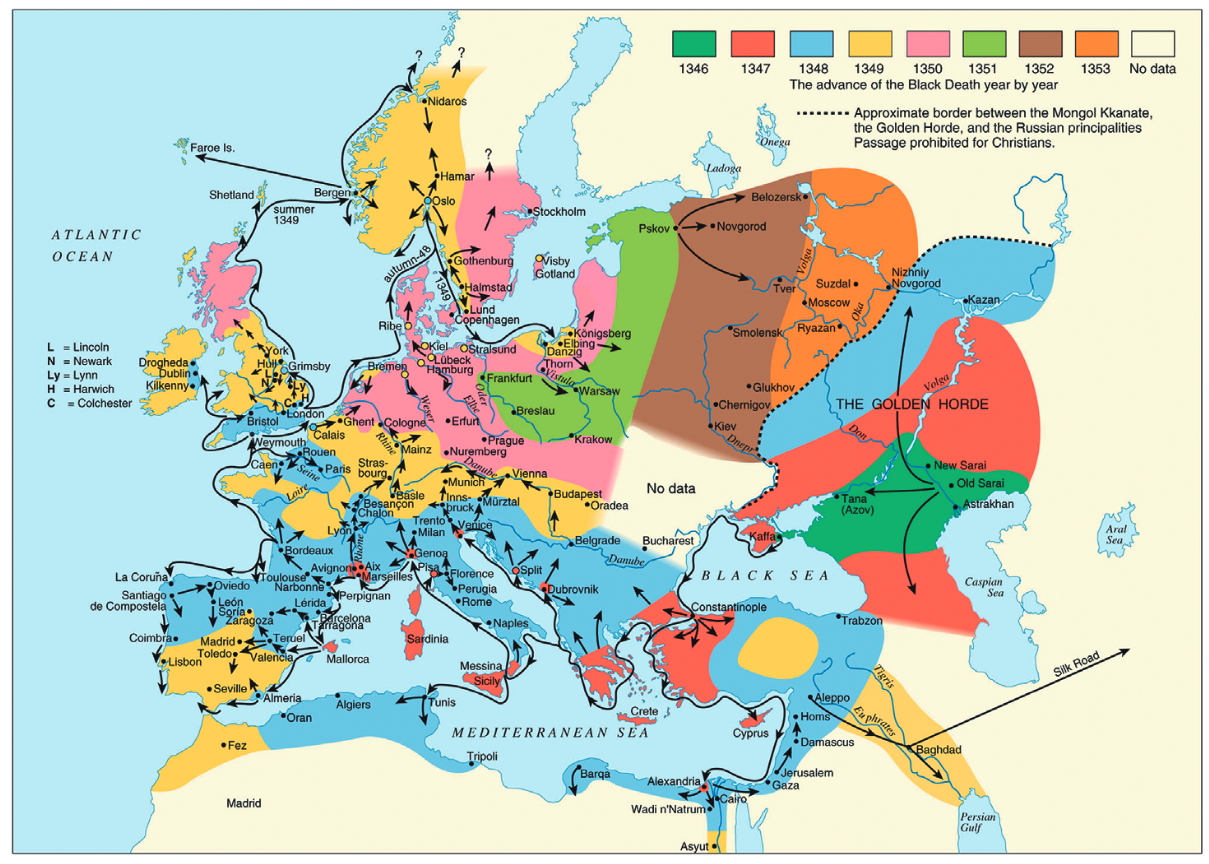
\includegraphics[width=\imsizeL]{Black_Death.png}
    \caption[Mapa de la peste negra en Europa.]{Mapa de la peste negra en Europa \cite{black_death}.}
    \label{fig:Black_Death}
\end{figure}

En resumen, el mecanismo de transmisión era el siguiente: algunas de las pulgas sufrían un bloqueo estomacal luego de alimentarse de una rata infectada, como 
consecuencia, estas pulgas comenzaban a picar con mayor frecuencia de lo habitual dado que la sangre que ingerían no les llegaba a los intestinos para ser digerida. El punto 
crucial de la cadena de transmisión, reside en la existencia de dos poblaciones distintas de ratas, una resistente y otra que no lo es. La especie resistente era la responsable 
de mantener la enfermedad endémica albergando las pulgas infectadas. Mientras que la especia no resistente generaba una escasez de alimento para las pulgas, las cuales 
se veían forzadas a cambiar de huésped, en este caso, el humano. Finalmente, la enfermedad se transmitía cuando las pulgas con bloqueo estomacal vomitaban sangre infectada
al picar a una persona \cite{black_death2}.


La plaga se introdujo a Europa por Italia en diciembre de 1347 y se extendió rápidamente, a un ritmo de 300 - 600 km por año \cite{Murray2003}. 
En la figura \ref{fig:Black_Death} se muestra la propagación espacio-temporal de la peste negra en Europa. Las rutas comerciales fueron las principales vías de 
propagación de la plaga.

\subsection*{Gripe Española}

La gripe española, por su parte, se extendió por todo el mundo entre 1918 y 1920, se estima que causó la muerte de una 40 millones de personas y entre un 25-30 \% de la 
población mundial padeció la enfermedad \cite{gripe2}. Se originó en Kansas, Estados Unidos, y se extendió por todo el mundo en menos de un año. Curiosamente, se denominó gripe
española simplemente porque España no participó en la Primera Guerra Mundial que acontecía simultáneamente, por lo tanto, no se censuraron los datos de la enfermedad.
La gripe española fue una pandemia de gripe de tipo A, causada por el virus H1N1. Fue la primera de tres pandemias causadas por este virus, la última de
las cuales ocurrió en 2009. 

A diferencia de otros virus de tipo A, que típicamente tienen mayor mortalidad sobre niños y ancianos, este virus impactó fuertemente sobre la población 
joven-adulta (20-40 años) \cite{gripe3}. El mecanismo de transmisión es como el de la gripe común, es decir, aéreo, por medio de gotitas de saliva que se expulsan al toser o estornudar.

Es interesante notar en este caso cómo el contexto histórico influyó en la propagación de la enfermedad. En 1918, la Primera Guerra Mundial estaba en su apogeo y 
muchos países se encontraban en medio de una crisis económica. Se piensa que la elevada tasa de transmisión de la enfermedad, con un número de reproducción básico entre 
2 y 3 \cite{gripe}, se debió a la enorme cantidad de tropas movilizadas por todo el mundo. Además, esto mismo sustentó mutaciones en el virus. 



\sect{Modelo SIR de campo medio}{sir_cm}

El modelo SIR describe la dinámica de tres grupos característicos de un sistema, denominados comúnmente como \textbf{S}usceptibles, \textbf{I}nfectados y
\textbf{R}ecuperados, de ahí su nombre. Es el modelo más simple para describir la propagación de una enfermedad 
infecciosa, fue propuesto originalmente hace casi un siglo, en 1927, por \textit{Kermack} y \textit{McKendrick} \cite{SIR}. 

El mismo está formulado de la siguiente manera: sean $S(t)$, $I(t)$ y $R(t)$ la fracción de susceptibles, infectados
y recuperados de una población dada a tiempo $t$ respectivamente, entonces, la dinámica de estos grupos está descrita por el siguiente sistema de
ecuaciones diferenciales ordinarias

\begin{align}
  \dv{S}{t}&=-\beta SI,\label{Seq}\\[.3cm]
  \dv{I}{t}&=\beta SI - \gamma I,\label{Ieq}\\[.3cm]
  \dv{R}{t}&=\gamma I.\label{Req}
\end{align}


Donde $\beta$ corresponde a una tasa de transmisión mientras que $\gamma$ corresponde a una tasa de recuperación.

Usualmente, la ecuación para $R$ (\ref{Req}) no se escribe, ya que puede ser reemplazada por la más simple $S+I+R=1$. Puede verse por inspección que el sistema de ecuaciones
(\ref{Seq} - \ref{Req}) cumple $\dv{S}{t}+\dv{I}{t}+\dv{R}{t}=0$.

Para entender por qué este simple sistema de ecuaciones (\ref{Seq} - \ref{Req}) podría describir la dinámica del problema observamos que el mismo 
está compuesto esencialmente por dos términos, el término de transmisión $\beta SI$ y el de recuperación $\gamma I$. Cualitativamente, resulta 
razonable que la magnitud de sujetos infectados por unidad de tiempo aumente con el producto de la cantidad de infectados y susceptibles, de ahí 
el término de transmisión. Por otro lado, la cantidad de infectados que se recuperan por unidad de tiempo es entendible que sea proporcional a la
misma cantidad de infectados y de ahí el término de recuperación. Por supuesto, es posible justificar esto de una manera más cuantitativa y precisa, para 
ver una derivación de estas ecuaciones consúltese \cite{keeling:infectious_diseases}.

A pesar de su simplicidad, este modelo (\ref{Seq} - \ref{Req}) no puede resolverse explícitamente. Es decir, no puede hallarse una expresión analítica exacta
para $I(t)$ y $S(t)$ que nos permita anticipar la cantidad de infectados que habrá a tiempo $t$ dadas las condiciones iniciales $I(0)=I_0$ y $S(0)=S_0$\footnote{En realidad,
para ser precisos, en 2014 se encontró una solución analítica, en términos de una integral que debe resolverse numéricamente \cite{sir_sol}.}.
Por ello
es necesario recurrir a métodos numéricos para resolverlo. En la figura \ref{fig:SIR} se puede ver la evolución temporal de las variables del modelo 
resuelto numéricamente\footnote{Se utilizó Runge-Kutta de cuarto orden para la integración numérica \cite{Recipes}.} usando los parámetros $\beta=5$/semana y
$\gamma=1$/semana con condiciones iniciales $I_0=0.01$ y $S_0=0.99$. Se observa cómo la fracción de susceptibles decrece mientras la de infectados 
aumenta hasta llegar a un pico donde aproximadamente la mitad de la población está infectada. Luego los infectados comienzan a recuperarse y casi toda
la población termina en la clase $R$, de modo que la mayoría de la población atravesó la enfermedad.

\begin{figure}[h]
  \centering
  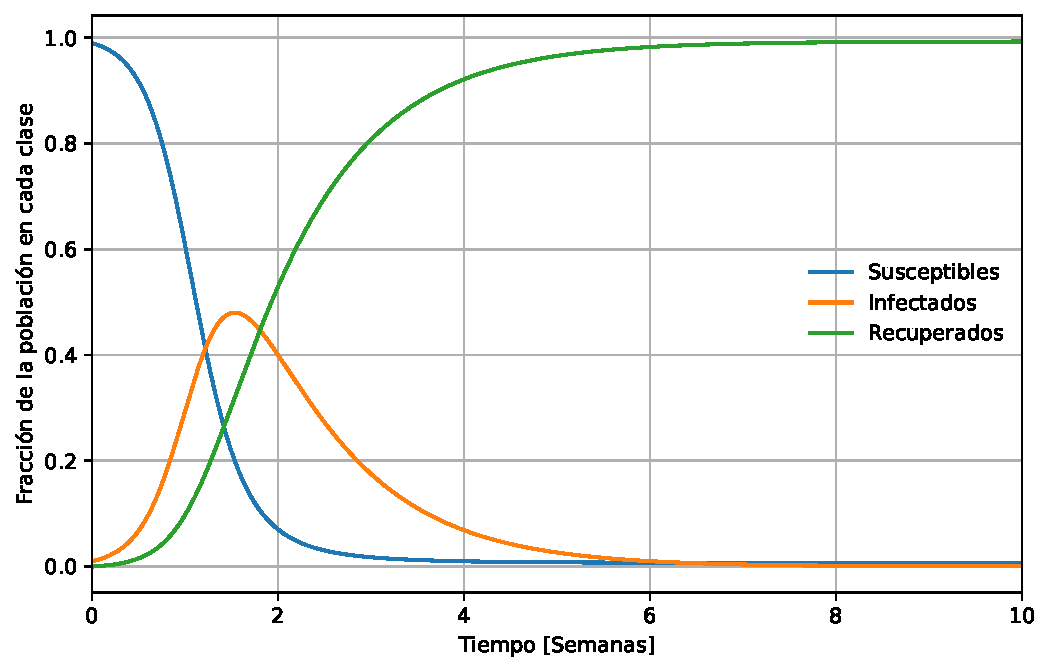
\includegraphics[width=\imsize]{SIR.pdf}
  \caption[Solución numérica del modelo S-I-R]{Evolución temporal de las variables del modelo resuelto numéricamente 
  con $\beta=~5$/semana, $\gamma=1$/semana, $I_0=0.01$ y $S_0=0.99$.}
  \label{fig:SIR}
\end{figure}


Es claro que la figura \ref{fig:SIR} no muestra toda la riqueza del sistema, ya que simplemente muestra la solución para un solo conjunto de parámetros y 
condiciones iniciales. Es decir, es de esperar que la dinámica difiera si por ejemplo la tasa de transmisión $\beta$ es menor. En particular, es de 
interés saber qué conjunto de parámetros $\beta$ y $\gamma$ favorecen o dificultan el progreso de la infección. Esto puede determinarse de manera sencilla pidiendo que $\dv{I}{t}<0$ 
al momento del brote de la infección. De esto resulta que si $S_0<S_c=\gamma/\beta$ para cualquier $I_0>0$ entonces la infección no progresa. 
Este es un resultado conocido, obtenido por Kermack y McKendrick (1927).

El cociente $\gamma/\beta$ es la tasa de recuperación relativa, sin embargo, su recíproco le quita todos los méritos, $R_0=~\beta/\gamma$ 
conocido en epidemiología comúnmente como el número de reproducción básico, el cual describe la media de personas infectadas por un individuo 
infectado. Dado que usualmente $S_0\approx 1$, la condición para que la infección perezca se lee ahora en función de $R_0$
simplemente como $R_0 < 1$. Lo cual resulta natural, si un infectado infecta en promedio a menos de una persona en lo que cursa la enfermedad entonces 
la infección no se propaga. En la figura \ref{fig:SIR_R} se puede ver la evolución temporal de las variables del modelo resuelto numéricamente con distintos 
números de reproducción básico $R_0$. Se observa que en la medida que $R_0 \to 1$ la magnitud del máximo de infección va decreciendo, mientras que cuando $R_0 = 1$ la 
cantidad de infectados solo decrece en el tiempo hasta llegar a cero. Lo mismo sucede si $R_0<1$.

Es importante no confundir el número de reproducción básico $R_0$ con el número de reproducción efectivo $R_e(t)$, el primero considera que todos los individuos de la 
población son susceptibles, mientras que el segundo no y varía con el tiempo, se define como $R_e(t)=\beta S(t)/\gamma$. Este probablemente sea el indicador epidemiológico 
más usado e importante. De manera similar que con $R_0$, se puede ver que si $R_e(t) < 1$ entonces la tasa de infección $\dv{I}{t}\left(t\right)$ es decreciente.

\begin{figure}[h]
  \centering
  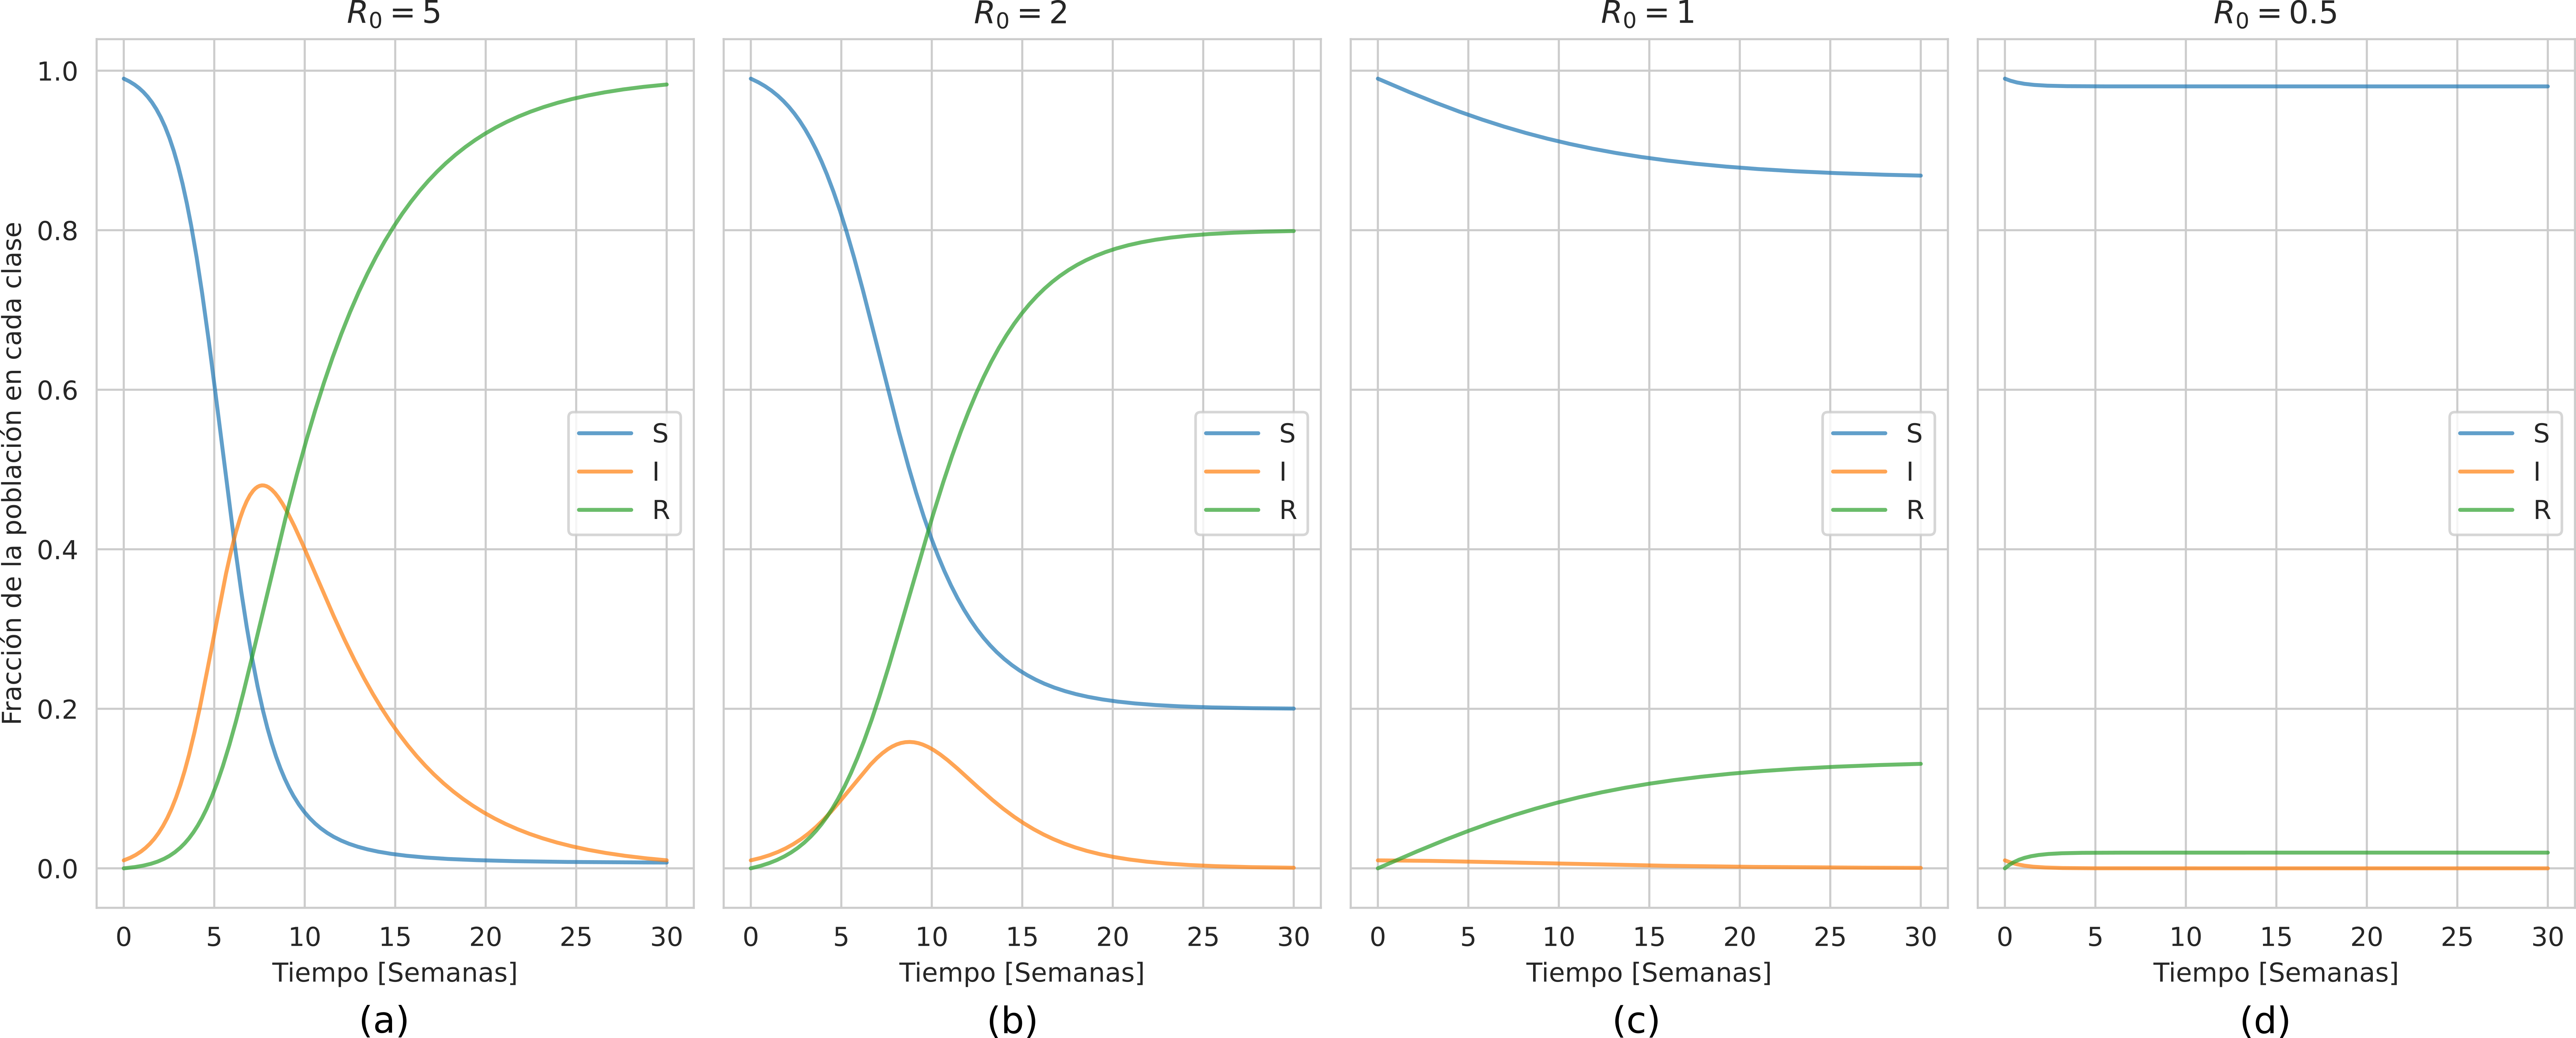
\includegraphics[width=\imsizeL]{SIR_R.png}
  \caption[Solución numérica del modelo S-I-R con distintos valores de $R_0$]{Evolución temporal de las variables del modelo resuelto numéricamente con (a) 
  $R_0 = 5$, (b) $R_0 = 2$, (c) $R_0 = 1$ y (d) $R_0 = 0.5$.}
  \label{fig:SIR_R}
\end{figure}

Otra cantidad de interés es la fracción de la población que no se contagió nunca. Es decir, cuánto vale el límite $\lim_{t \to \infty} S(t) \equiv S(\infty)$. De la figura 
\ref{fig:SIR_R} se puede ver que cuando $R_0=5$ la fracción de la población que no se 
contagia es muy cercana a cero, pero distinta a cero en fin. Mientras que cuando $R_0 = 2$, pareciera que $S(\infty) \to 0.2$. Para responder esta pregunta de manera más 
general podemos tomar la ecuación \ref{Seq}, dividirla por \ref{Req} y luego integrar para obtener una expresión de $S$ en función de $R$. De esto resulta que,
$$S(t) = S_0 e^{-R_0R(t)},$$
tomando el límite correspondiente, usando $\lim_{t \to \infty}R(t)\equiv R(\infty)$ y que $R(\infty) = 1 - S(\infty)$, resulta la siguiente ecuación trascendental 
para $S(\infty)$
\begin{align}
  S(\infty) &= S_0 e^{-R_0 (1 - S(\infty))},\nonumber \\
  0 &= S(\infty) - S_0 e^{-R_0 \left(1 - S(\infty)\right)}.  \label{Sinf}
\end{align}
Puede verse que si $S(\infty) = S_0$, entonces el miembro derecho de \ref{Sinf} es positivo, mientras que si $S(\infty) = 0$, es negativo. De modo que la ecuación 
\ref{Sinf} tiene una solución para $S(\infty)$ entre $0$ y $1$. Es decir, sin importar qué tan grande sea el número de reproducción básico $R_0$, o bien, qué tan 
contagiosa sea la enfermedad, siempre existe una fracción de la población que no se contagia.

Es importante señalar brevemente las virtudes y fundamentalmente las hipótesis bajo las que se presenta este modelo. La ventaja más notable es la 
simplicidad y el carácter didáctico del mismo, que como vimos, permite definir y asimilar conceptos generales asociados a la problemática de manera sencilla.
Esta simplicidad, sin embargo, viene acompañada de hipótesis que en ocasiones resultan restrictivas y poco realistas en lo que respecta a una dinámica
tan compleja como la de una epidemia. Por ejemplo, se ignoran efectos de demografía los cuales
pueden tener un impacto apreciable sobre la dinámica a escalas temporales extensas propias de una endemia. Además, se trata de un modelo de campo medio, 
donde se asume que cada sujeto de la población interactúa con todos los demás, es decir, desprecia heterogeneidades que puedan surgir de la edad, el 
espacio o aspectos de comportamiento. Adicionalmente, supone que individuos que pasaron por la enfermedad adquieren inmunidad para toda la vida y que
un sujeto inmedianamente infectado puede infectar a otro. Por supuesto, esto no desmerece en nada al modelo, el cual sigue siendo extremadamente útil como primera 
aproximación al modelado de este tipo de sistemas complejos, simplemente es importante recordar las hipótesis sobre las que se trabaja para evitar posibles confusiones.

Por último, es de interés mencionar que si bien el enfoque ha estado hasta ahora centrado en una descripción epidemiológica, es posible extender este 
mismo modelo de manera sencilla a otras problemáticas. En particular, puede asociarse rápidamente el modelo SIR con la dinámica
de un incendio en un bosque. Donde los <<susceptibles>> son los árboles que pueden incendiarse, los <<infectados>> son los árboles en 
llamas y los <<recuperados>> los árboles que ya han sido quemados y no pueden volver a incendiarse.
 

\sect{Modelo SIR de reacción-difusión homogéneo}{modeloRDHo}

De manera general las ecuaciones de reacción-difusión sobre un medio isotrópico son aquellas que pueden escriberse como
\begin{equation}
  \pdv{\vb{u}}{t} = \vb{f} + \div(D\grad{\vb{u}}),
\end{equation}
donde $\vb{u}$ es un campo vectorial que dependende de la posición $\mathbf{x}$ y el tiempo $t$, $\vb{f}$ es el término de reacción, que es función de 
$\vb u$, $\vb x$ y $t$, mientras que $\div(D\grad{\vb{u}})$ es el término de difusión, donde D es la matriz de difusión que puede ser función de $\vb x$.
Este tipo de ecuaciones han sido ampliamente estudiadas \cite{keeling:infectious_diseases,Murray2002,Murray2003,crank1979mathematics} y se denominan así porque originalmente 
se utilizaron para estudiar la dinámica de reactivos químicos.\cite{turing52the}

En lo que respecta al modelo SIR de reacción-difusión que nos interesa a nosotros, este puede escribirse de manera sencilla agregando 
el término difusivo a las ecuaciones (\ref{Seq} - \ref{Req}), dejando de lado la ecuación para $R$, esto es 
\begin{align}
  \partial_t S &=-\beta SI + D_{S} \laplacian{S},\label{Seqdif}\\[.3cm]
  \partial_t I &=\beta SI - \gamma I + D_{I} \laplacian{I}.\label{Ieqdif}
\end{align}

Donde ahora $S$, $I$ y $R$ son funciones de la posición $(x,y)$ en un espacio bidimensional además del tiempo $t$, de modo que ahora 
se cumple $S(x,y,t)+I(x,y,t)+R(x,y,t)=1$ para todo $(x,y,t)$. En este nuevo modelo 
(\ref{Seqdif} - \ref{Ieqdif}) los términos difusivos dan lugar a una transmisión local de la infección. Es decir, abandonamos 
el modelo de campo medio que teníamos en la sección \ref{sec:sir_cm} donde todos los individuos podían interactuar entre sí.

Hemos supuesto que los coeficientes de difusión $D_{S}$ y $D_{I}$ son independientes de la posición y que la matriz $D$ es diagonal 
dejando de lado la posibilidad de difusión cruzada. Adicionalmente, tanto $\beta$ como $\gamma$ son 
independientes de la posición, dando lugar a un medio totalmente homogéneo, todos los puntos del espacio son equivalentes en términos de transmisión. Esta 
es una característica crítica a remarcar, ya que en la sección \ref{sec:modeloRDHe} presentamos el correpondiente modelo heterogéneo, donde 
el medio puede adquirir un carácter desordenado, que es el foco de estudio de este trabajo.

A continuación se muestran algunos resultados interesantes asociados a este modelo que serán de interés a la hora de compararlo con su versión heterogénea.

\ssect{Soluciones de onda}{ondas}

Dada una fracción de infectados inicial $I(x,y,0)$ y una fracción de susceptibles 
distribuída homogéneamete $S(x,y,0)=S_0$, se quiere saber cómo es la evolución espacio-temporal de la fracción de infectados $I(x,y,t)$. En la problemática 
de incendios la idea sería la misma, pero cambiando infectados por, digamos, incendiados. 

Nuevamente, no es posible resolver las ecuaciones \ref{Seqdif} y \ref{Ieqdif} de manera exacta, sin embargo, es posible estudiar qué condiciones deben 
satisfacerse para que cierto tipo de soluciones puedan existir. En particular, nos interesa estudiar bajo qué condiciones podría existir una solución de onda 
y qué características tendría.

Para ello proponemos una solución de onda plana donde 
\begin{align}
  S(x,y,t)&=S(z), & I(x,y,t)&=I(z), &  z&=x-ct, \label{wave}
\end{align}
que representa una onda de infección viajando en la dirección $x$ positiva con una velocidad $c>0$. Reemplazando \ref{wave} en \ref{Seqdif} y \ref{Ieqdif}, resulta el 
siguiente sistema de ecuaciones no lineales,

\begin{align}
  D_S S''+ cS'-\beta IS &=0,\label{Sz} \\[.3cm] D_I I'' + cI' + \beta I(S-\gamma/\beta)&=0, \label{Iz}
\end{align}
donde las primas indican derivadas respecto de $z$. Como es habitual, este sistema tampoco puede resolverse explícitamente, sin embargo, imponiendo las 
siguientes condiciones para las soluciones\footnote{Se utiliza la siguiente notación por simplicidad, dada una función $f(z)$, 
\[\lim_{z\to\pm\infty}f(z)\equiv f(\pm\infty)\]}
\begin{align*}
  I(\pm\infty)&=0,   &  S(\infty) &= S_0,  & S(-\infty) &= S_1,   
\end{align*}
donde $S_1$ sería la fracción de susceptibles que deja la onda por detrás, es posible linearizar la ecuación \ref{Iz} para $z$ donde $S(z)\approx S_0$,
es decir, sobre el perfil frontal de la onda. De lo cual resulta,
\begin{equation}
  D_I I'' + cI'+\beta I(S_0-\gamma/\beta)=0,\label{Idez}
\end{equation}
que tiene una solución $I(z)\propto e^{-\lambda z}$, con $\lambda$ satisfaciendo,
\[D_I \lambda^2 - c \lambda +\beta(S_0-\gamma/\beta)=0,\]
es decir,
\[\lambda = \frac{c}{2D_I}\pm \sqrt{(c/2D_I)^2-\frac{\beta}{D_I}(S_0-\gamma/\beta)}.\]
Debemos imponer además que $\lambda \in \mathds R$ con $\lambda>0$, de otra manera la solución no sería autoconsistente. Al imponer que $\lambda>0$ 
resulta $\gamma/\beta<S_0$, que es la misma condición que habíamos obtenido en la sección \ref{sec:sir_cm} para que la infección progrese, 
mientras que ahora es una condición necesaria para la existencia de soluciones onda, las cuales darían lugar a la 
propagación de la infección, por lo menos resulta concordante. Más interesante quizás, es la condición $\lambda \in \mathds{R}$, de la cual resulta que 
\begin{align*}
  0\leq&(c/2D_I)^2-\frac{\beta}{D_I}(S_0-\gamma/\beta),\\[.3cm]
  c\geq&2\sqrt{D_I\beta(S_0-\gamma/\beta)}\equiv c_0,
\end{align*}
dando así una velocidad mínima $c_0$ para la existencia de la onda. Veremos en la sección \ref{S:aleatorios} que la velocidad de propagación es en realidad
muy cercana a la mínima encontrada aquí $c_0$. Tomando esto por cierto, el perfil frontal de la onda de infección está dado por 
\begin{equation}
  I_f(z)\propto \exp[-\frac{c_0}{2D_I}z].\label{larika2}  
\end{equation}

Haciendo una cuenta equivalente para el perfil posterior de la onda donde $S(z)\approx S_1$, hay que resolver la ecuación análoga a \ref{Idez}, 
$D_I I'' + cI'+\beta I(S_1-\gamma/\beta)=0$, de esto resulta 

\begin{align}
  I_p(z)&\propto \exp[\left(-\frac{c_0}{2D_I}+\sqrt{(c_0/2D_I)^2-\frac{\beta}{D_I}(S_1-\gamma/\beta)}\right)z], \label{larika} \\[.3cm]
  I_p(z)&\propto \exp[\left(-\frac{c_0}{2D_I}+ \sqrt{\frac{\beta}{D_I}(S_0-S_1)}\right)z].
\end{align}
De la ecuación \ref{larika} se ve que es necesario que $\gamma/\beta>S_1$, dado que debe satisfacerse $I_p(-\infty) = 0$, de modo que en resumen se tiene la siguiente relación
\[S_0>\gamma/\beta>S_1>0,\]
es decir, que la fracción de susceptibles que quedan tras el paso de la onda no es suficiente para activar una onda de retroceso ya que $S_1<\gamma/\beta$.

En resumen, se obtuvieron expresiones analíticas aproximadas del perfil frontal y posterior que tendría una solución de onda, ecuaciones \ref{larika2} 
y \ref{larika} respectivamente, las cuales dan a entender que el perfil completo de la onda es asimétrico. Se determinó a su vez la velocidad de propagación de la onda $c_0=2\sqrt{D_I\beta(S_0-\gamma/\beta)}$ y se estableció la 
jerarquía $S_0>\gamma/\beta>S_1>0$ para la existencia de la onda.

\ssect{Soluciones en sistema de reacción-difusión-convección}{SIRrdc}

En este trabajo exploramos algunos resultados sobre un modelo SIR como el presentado en la sección \ref{sec:modeloRDHo} pero con un término adicional de convección. Esto es,
\begin{align}
  \partial_t S & = -\beta SI + D_S \laplacian{S} \\
  \partial_t I &= \beta SI + D_I \laplacian{I}- \mathbf{v} \cdot \nabla I
\end{align}
donde $\mathbf{v}$ es un campo vectorial. En términos epidemiológicos no es fácil dar una interpretación a este campo vectorial, sin embargo, podría interpretarse 
como un campo de migración de individuos infectados de un lugar a otro y la dirección de $\mathbf{v}$ sería la dirección de la migración, en tanto que su magnitud 
sería la velocidad de migración. Pensando en incendios es más sencillo motivar este término de convección, pues se podría interpretar como el campo de viento. 

Ahora bien, se puede ver que este modelo también tiene soluciones de onda cuando $\mathbf{v}$ es constante. Sin perder generalidad podemos tomar $\mathbf{v}=(v,0)$ con 
$v>0$, de modo que la ecuación de evolución para $I$ queda
\begin{equation}
  \partial_t I = \beta SI + D_I \laplacian{I}- v \partial_x I.
\end{equation}
Pasando las ecuaciones a un sistema de coordenadas que se mueve con la velocidad $v$, es decir, $x'=x-vt$, se obtiene 

\begin{equation}
  \partial_t I = \beta SI + D_I \laplacian{I},
\end{equation}
es decir, recuperamos el sistema de reacción-difusión que estudiamos antes. Tomando el desarrollo de la sección anterior se obtiene en este caso que la velocidad de propagación 
del frente de infección es 
$$c = c_0 + v,$$
mientras que si tomamos viento en contra $\mathbf{v} = (-v,0)$ se tiene,
$$c = c_0 - v.$$
Lo interesante del caso con viento en contra es que debemos pedir que $c>0$ de lo cual surge un nuevo valor crítico para el umbral de propagación. Es decir,

\begin{align*}
  c &> 0 \\
  2\sqrt{D_I\beta(S_0-\gamma/\beta)}\ - v &> 0 \\
  \sqrt{D_I\beta(S_0-\gamma/\beta)} &> v/2 \\
  \beta &> \frac{1}{S_0}(\frac{v^2}{4D_I}+\gamma) \equiv \beta_c, 
\end{align*}
donde $\beta_c$ es el umbral de propagación para el caso con viento en contra.




\sect{Modelo SIR de reacción-difusión heterogéneo}{modeloRDHe}

En esta sección presentamos el modelo que estudiamos con profundidad en este trabajo junto a algunas descripciones estadísticas del mismo que se usarán 
posteriormente. 

Esencialmente las ecuaciones son las mismas que \ref{Seqdif} y \ref{Ieqdif} con la salvedad de que ahora introducimos hetereogeneidad en el medio poniendo 
una tasa de transmisión $\beta_{\vb{r}}$ dependiente de la posición. Por completitud escribimos las ecuaciones nuevamente aquí,
\begin{align}
  \pdv{S}{t}&=-\beta_{\vb{r}} SI + D_{S} \laplacian{S}  ,\label{Seqfinal}\\[.3cm]
  \pdv{I}{t}&=\beta_{\vb{r}} SI - \gamma I + D_{I} \laplacian{I}.\label{Ieqfinal}
\end{align}

Una tasa de transmisión $\beta_{\vb{r}}$ de este tipo podría utilizarse, por ejemplo, para estudiar el efecto de la vacunación sobre la población. Esto es 
entendible dado que se espera que los lugares donde hay población vacunada la tasa de transmisión sea menor ya que hay menos individuos susceptibles para
infectarse. Otra alternativa apuntaría a describir lugares donde la tasa de transmisión es más baja por un efecto de densidad poblacional. 
En cuanto a la propagación de incendios podría interpretarse de manera similar como una variación de la densidad de vegetación en el espacio, lo cual 
facilitaría o no la transmisión de las llamas.

\subsection{Problema y observables}
\label{Problema}

Vamos a centrarnos en estudiar el frente de infección/incendio en un espacio cuadrado de longitud $L$, 
con $x,y \in [0,L-1]$, y condiciones iniciales
\begin{align*}
  I(x,y,0)=&I_0, & S(x,y,0)=&1-I_0,
\end{align*}
con $x\in(0,\delta x)$ y 
\begin{align*}
  I(x,y,0)=&0, & S(x,y,0)=&S_0,
\end{align*}
para $x\in[\delta x,L-1)$. Adicionalmente, se tienen condiciones de contorno de Dirichlet en la dirección $x$,
\begin{align*}
  I(0,y,t)=I(L-1,y,t)=S(0,y,t)=S(L-1,y,t)=0. 
\end{align*}
Y condiciones periódicas en la dirección $y$, 
\begin{align*}
  I(x,0,t)=&I(x,L-1,t) & S(x,0,t)=&S(x,L-1,t). 
\end{align*}
Estas condiciones iniciales y de contorno dan lugar a un único frente de onda propagándose en la dirección $x$, lo cual resulta conveniente para realizar un análisis 
estadístico a partir de ciertos observables, los cuales se definen a continuación.

Para caracterizar las fluctuaciones espaciales y temporales del frente de infección/incendio, definimos el campo de desplazamiento del frente $u(y,t)$ como
\begin{equation}
  \max_{x\in(0,L-1)}\{I(x,y,t)\}=I(u(y,t),y,t).\label{campo}
\end{equation}
Es decir, $u(y,t)$ es la posición en $x$ del máximo de la fracción de infectados/incendiados para un dado $y$ en el instante $t$. Se define a su vez el centro de masa
de $u(y,t)$,
\begin{equation}
  u_{cm}(t)\equiv\langle u(y,t)\rangle_{y},\label{centromasa}
\end{equation}
donde $\langle...\rangle_{y}$ indica el promedio sobre la coordenada $y$. El valor medio de la amplitud máxima de $I(x,y,t)$ sobre $u(y,t)$ es,
\begin{equation}
  I_{max}(t)=\langle I(u(y,t),y,t)\rangle_{y}.\label{maximo}
\end{equation}
Por otro lado, la velocidad media de la onda de propagación se define como,
\begin{equation}
  c\equiv\langle\dot{u}_{cm}(t)\rangle_{t}.\label{velocidad}
\end{equation}
donde $\langle...\rangle_{t}$ indica promedio sobre el tiempo. De manera similar, la amplitud media del frente de propagación es
\begin{equation}
  I_{max}=\langle I_{max}(t)\rangle_{t}.  \label{Imax}
\end{equation} 
Las fluctuaciones del frente de onda pueden ser caracterizadas definiendo la rugosidad del mismo como la desviación estándar de $u(y,t)$,
\begin{equation}
  w(t)^2\equiv\langle[u(y,t)-u_{cm}(t)]^2\rangle_{y},\label{rugosidad}
\end{equation}  
o con el factor de estructura,
\begin{equation}
  S(q)\equiv\langle|u(q,t)|^2\rangle_{t},\label{factor}
\end{equation}
donde $u(q,t)$ es la transformada de Fourier sobre el espacio de $u(y,t)$.
Por último, estaremos interesados en observar el perfil de la onda de propagación, estos es,
\begin{equation}
  f_{I}(x)=\langle I(x-u(y,t),y,t)\rangle_{y,t}.\label{perfil}
\end{equation}

En el capítulo \ref{Simulaciones} utilizaremos los observables definidos aquí como principales herramientas para caracterizar y comparar de manera cuantitativa
los efectos que tienen distintas heterogeneidades, introducidas mediante $\beta_{\vb r}$, sobre la dinámica del problema. 







